
\section{Representing bytecode programs as control flow graphs}\label{prelim}

This section will introduce a formalization of an unstructured program in terms of a control flow graph.
The notion of a loop in a bytecode program will be also defined.
Performing analysis on programs written in  structured languages, is usually easier than performing the same analysis 
on unstructured programs. In particular, source loops in a method body correspond to a syntactic construction which is not the 
case for loops in methods on bytecode level. In order to discover a loop in a bytecode program we first need to define 
what is a bytecode program. Note that in the following, by a  bytecode program we mean a method body.

Every method \methodd \ has an array of bytecode instructions \methodd.\body \  which we already introduced in Section \ref{clazz}.
The $k-th$ instruction in the bytecode array $\methodd.\body$ is  denoted with $\methodd.\body[k]$.
 We assume that the method body has exactly one entry point
 (an entry point instruction is the instruction at which an execution of a method starts) which is the first
 element in the method body
$\methodd.\body[0]$.
The array of bytecode instructions of a method \methodd \ determine an oriented graph $G( V , \execRel ) $ in which the vertices are the instructions of the method body,
i.e. $$ V = \{ ins \mid \exists k,  0 \leq k < \methodd.\body.length \wedge ins = \methodd.\body[k] \}$$
The set of edges $\execRel$ is a relation between the vertices elements
$$ \execRel : V * V $$ and is defined  as follows:
$$ (\methodd.\body[j], \methodd.\body[k]) \in \execRel \iff 
   \begin{array}{l} \methodd.\body[j] \neq \return \wedge( \\
                    \methodd.\body[j] = \ifCond \ k \vee \\
		    \methodd.\body[j] = \goto \ k \ \vee \\
		    \methodd.\body[j] \neq \goto \Rightarrow  k = j+1)
   \end{array}$$
 i.e. there is an edge between two vertices $\methodd.\body[j]$ and  $\methodd.\body[k]$ if they may execute immediately one after another.
In the following, we will rather use the infix notation $\methodd.\body[j] \execRel \methodd.\body[k]$.


We assume that the control flow graph of every method is reducible, i.e. every loop has exactly one entry point. This actually is admissible
as it is rarely the case that a compiler produce a bytecode with a non reducible control flow graph and the practice shows that even hand written
code is usually reducible. However, there exist algorithms to transform a non reducible control flow graph into a reducible one. 
For more information on program control flow graphs, the curious reader may refer to \cite{ARUCom1986}.
The next definition identifies backedges in the reducible control flow graph ( intuitively, the edge that goes 
from an instruction in a given loop in the control flow graph to the loop entry)  with the special execution relation $\execRel^l$ as follows:
 
\begin{defLoop}[Backedge Definition]
\label{defLoop}
Let's have the method \methodd \ with body \methodd.\body \ which determine the control flow graph $G(V, \execRel) $.  $G$ is such that 
the vertice  $\methodd.\body[0]$ does not have predecessors and any path that reaches any other instruction in the graph
passes through $\methodd.\body[0]$. In such a graph $G$, we say that $\ins{loopEntry}$ is a loop entry instruction and $\ins{f}$ is a loop end instruction
 of the same loop if the following conditions hold:
\begin{itemize}
\item every path in the control flow graph starting at the entry point $\methodd.\body[0]$  that reaches $\ins{f}$, passes before reaching $\ins{f}$
 through  $\ins{loopEntry}$ 
\item there is a path in which $\ins{loopEntry}$  is executed immediately after the execution of $\ins{f}$ ( $\ins{f} \execRel \ins{loopEntry}$)
\end{itemize}
We denote the execution relation between $\ins{f}$ and  $\ins{loopEntry}$ with \\
$\ins{f} \execRel^l \ins{loopEntry}$ and we say that $  \execRel^l $  is a backedge. 
\end{defLoop}
We illustrate the upper definition with the control flow graph of the example from Fig. \ref{replaceSrc} in Fig. \ref{ctrlflow}.
In the figure, we rather show the execution relation between basic blocks (a standard notion denoting a sequence of instructions where
only the last one may be a jump and the first may be a target of a jump) the execution relation between the 
intstructions in a block being evident.


\begin{figure}[ht!]
\begin{center}
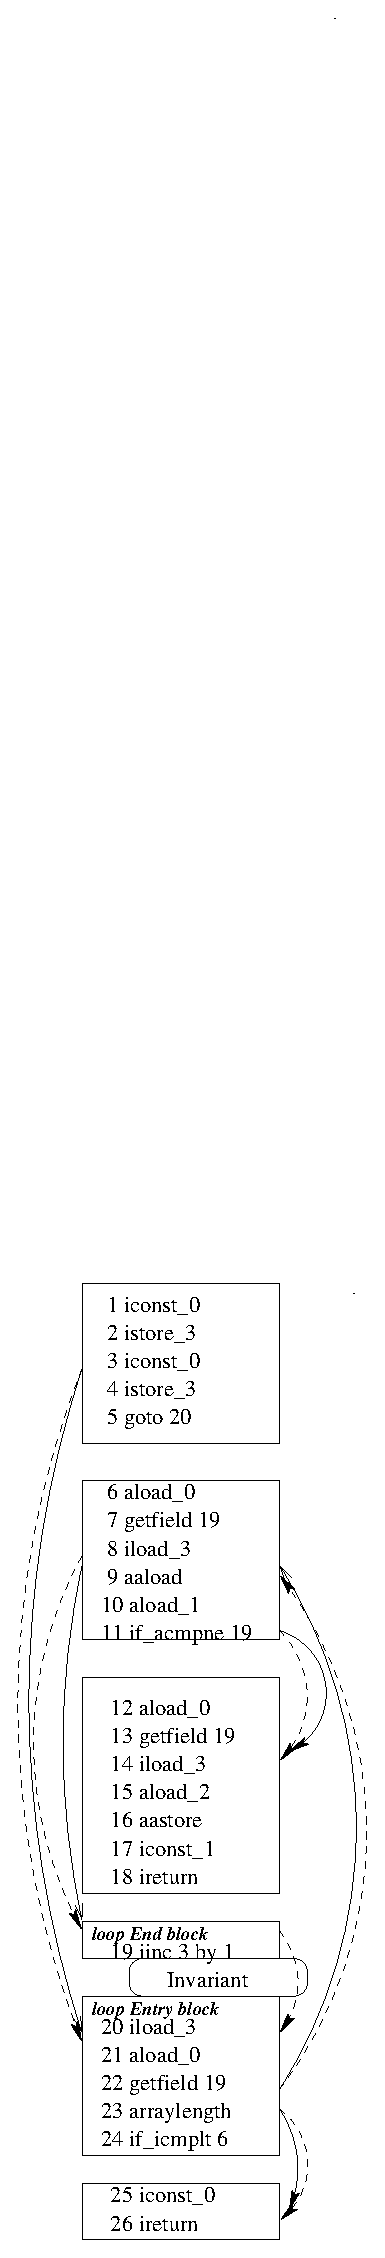
\epsfig{file=bytecode.eps, width=\linewidth}
\caption{The control flow graph of the source program from Fig.\ref{replaceSrc} }
\label{ctrlflow}
\end{center}
\end{figure}

The next lemma states a property about execution paths in a control flow graph that contains backedges. This lemma will be used in the proof of correctness
of our calculus in section \ref{proof}.
\begin{propPath} \label{propPath}
 Let's have a control flow graph with an entry point instruction $\methodd.\body[0]$ and two instructions $\ins{loopEntry}$ and  
 $\ins{f}$ such that  \\
 $\ins{f}~\execRel^l~\ins{loopEntry}$. If there exists an execution path $P$ from $\methodd.\body[0]$ to  $\ins{f}$:   $P~=~\methodd.\body[0] \execRel^{+} \ins{f}$
 then there exists a subpath which is a prefix of $P$  $subP = \methodd.\body[0] \execRel^{*} \ins{loopEntry}$ such that $\ins{f} \notin  \ subP  $ 
 \end{propPath} 


%Once we have defined what a loop means in a control flow graph, we want also to define what a loop invariant means. 

%\begin{defInv}[Loop Invariant]\label{defInv}
%An invariant is an assertion which accompanies a backedge  in a bytecode control flow graph. Every backedge is accompanied 
%by an invariant. We denote an invariant with $\invariant$. If a backedge  $\execRel^{l}$ is accompanied by an invariant $\invariant$ 
%then $\invariant$ holds in every state in which an execution path passes through  the edge $\execRel^{l}$.    
%\end{defInv}

%We also assume that loop entries are provided with the locations \modifLoop \ that a loop may modify. 
%The interest of having the set of the locations that may be modified by a loop will be seen later when defining the weakest precondition
%predicate transformer.


% \begin{defModif}[Loop Modifies]\label{defModif} Every loop entry instruction $\ins{loopEntry}$ with
%a set of locations $\modifLoop = \{ mod_i \mid  i = 1 .. s\}$ whose meaning is the following: any two states $state_1, state_2 $  in which
% the instruction $ \ins{loopEntry}$ executes agree on local variables and the heap modulo the locations that are in the list \modifLoop.
%We denote the equality between  $state_1, state_2 $   modulo the modifies locations like this 
% $ state_1 =^{\modifLoop } state_2$
%\end{defModif}

